\documentclass[12pt,letterpaper]{article}
\usepackage[utf8]{inputenc}
\usepackage[spanish]{babel}
\usepackage{graphicx}
\usepackage[left=2cm,right=2cm,top=2cm,bottom=2cm]{geometry}
\usepackage{graphicx} % figuras
% \usepackage{subfigure} % subfiguras
\usepackage{float} % para usar [H]
\usepackage{amsmath}
%\usepackage{txfonts}
\usepackage{stackrel} 
\usepackage{multirow}
\usepackage{enumerate} % enumerados
\renewcommand{\labelitemi}{$-$}
\renewcommand{\labelitemii}{$\cdot$}


% \author{}
% \title{Caratula}
\begin{document}

% Fancy Header and Footer
% \usepackage{fancyhdr}
% \pagestyle{fancy}
% \cfoot{}
% \rfoot{\thepage}
%

% \usepackage[hidelinks]{hyperref} % CREA HYPERVINCULOS EN INDICE

% \author{}
\title{Caratula}

\begin{titlepage}
\begin{center}
\large{UNIVERSIDAD PRIVADA DE TACNA}\\
\vspace*{-0.025in}
\begin{figure}[htb]
\begin{center}

\includegraphics[width=8cm]{./Imagenes/logo}
\end{center}
\end{figure}
\vspace*{0.15in}
INGENIERÍA DE SISTEMAS  \\

\vspace*{0.5in}
\begin{large}
TITULO:\\
\end{large}

\vspace*{0.1in}
\begin{Large}
\textbf{Trabajo Encargado - Proyecto Final} \\
\end{Large}

\vspace*{0.3in}
\begin{Large}
\textbf{CURSO:} \\
\end{Large}

\vspace*{0.1in}
\begin{large}
BASE DE DATOS II\\
\end{large}

\vspace*{0.3in}
\begin{Large}
\textbf{DOCENTE(ING):} \\
\end{Large}

\vspace*{0.1in}
\begin{large}
 Patrick Cuadros Quiroga\\
\end{large}

\vspace*{0.2in}
\vspace*{0.1in}
\begin{large}
Integrantes: \\
\begin{flushleft}
Percy Taquila Carazas\hfill	(2018061088) \\
Apaza Mamani Edward\hfill	(2018060915) \\
\end{flushleft}
\end{large}
\end{center}

\end{titlepage}

\tableofcontents % INDICE
\thispagestyle{empty} % INDICE SIN NUMERO
\newpage
\setcounter{page}{1} % REINICIAR CONTADOR DE PAGINAS DESPUES DEL INDICE


\section{Objetivos} 

\begin{itemize}
- Realizar la Instalación de un sistema de gestión de Base de Datos Oracle sobre el programa de virtualización (Hyper-V)con un sistema operativo Ubuntu Linux.\\
\end{itemize} 


\section{Requerimientos} 

\begin{itemize}
\subsection{Conocimientos}\\
- Conocimientos básicos de comandos Linux.\\\\


\subsection{Hardware}\\
- 01 procesador de doble núcleo o superior\\
- 4Gb de memoria física (RAM) o superior\\
- Disco duro con 100Gb de capacidad\\\\


\subsection{Software}\\
- Sistema Operativo Windows 10\\
- Instalador de Oracle Ubuntu(En DVD o archivo de tipo imagen .ISO).\\
- Instalador de Oracle Database (En DVD o archivo de tipo imagen .ISO).\\
- Hyper-V.
\end{itemize} 


\section{Pasos a seguir}

\begin{itemize}
\subsection{Instalación del Hyper-V}\\
- Nos dirigimos al buscador del Windows 10 y escribimos: 'Activar o desactivar las características de Windows'.\\
\end{itemize}

\begin{center}
	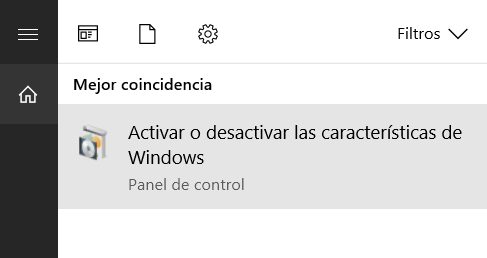
\includegraphics[width=8cm]{./Imagenes/1} 
\end{center}


\begin{itemize}
- Buscamos la opción llamada 'Hyper V', lo activamos la casilla y reiniciamos la pc.\\
\end{itemize}

\begin{center}
	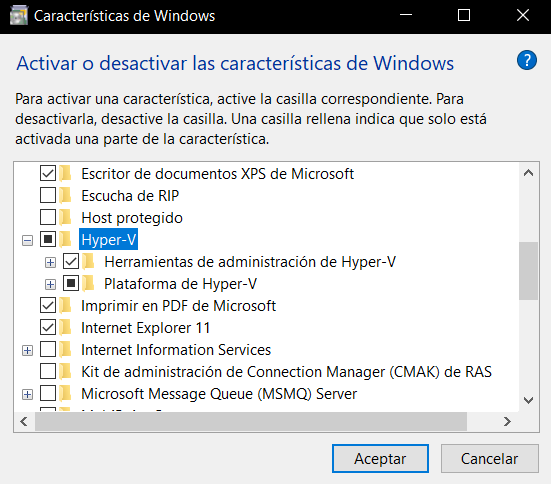
\includegraphics[width=8cm]{./Imagenes/2} 
\end{center}


\begin{itemize}
\subsection{Configuración del Hyper-V}\\
- Nos dirigimos a 'Administrador de conmutadores virtuales'. En la ventana que nos muestra
tenemos que elegir conmutador 'Interno', luego hacemos click en 'Crear conmutador virtual'.
\end{itemize}

\begin{center}
	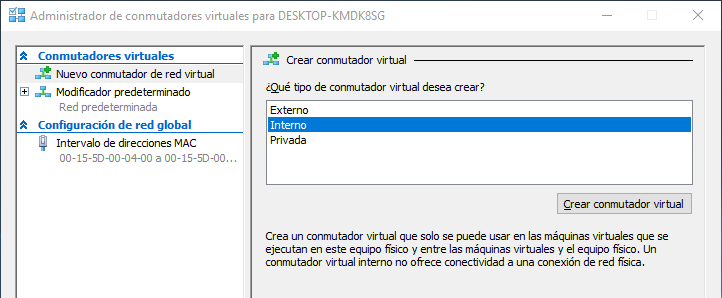
\includegraphics[width=10cm]{./Imagenes/3} 
\end{center}


\begin{itemize}
- Nos pedirá ingresar un nombre, ponemos el que deseamos. Verificamos si esta marcada la casilla
en 'Red interna' y damos click en 'Aceptar'.\\
\end{itemize}

\begin{center}
	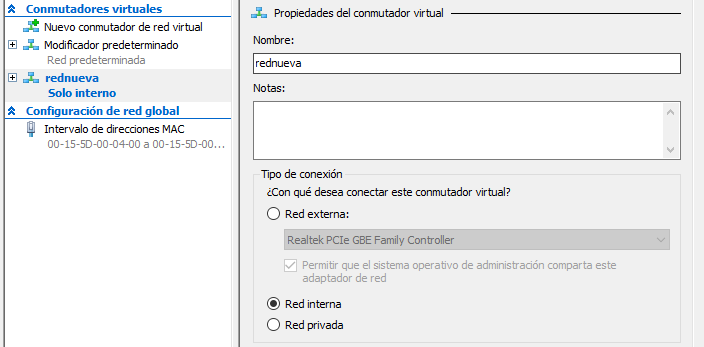
\includegraphics[width=10cm]{./Imagenes/4} 
\end{center}


\begin{itemize}

\subsection{Creación de la maquina virtual Ubuntu en Hyper-V}\\
- Hacemos click en 'Nuevo-Maquina virtual'. En la ventana que nos muestra ingresamos el nombre que deseemos poner a la maquina virtual, damos siguiente.
\end{itemize}

\begin{center}
	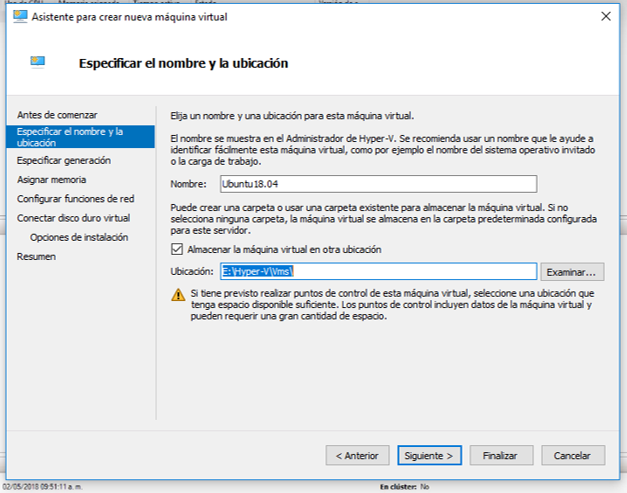
\includegraphics[width=10cm]{./Imagenes/7} 
\end{center}



\begin{itemize}
- Elegimos la generación 2\\
\end{itemize}

\begin{center}
	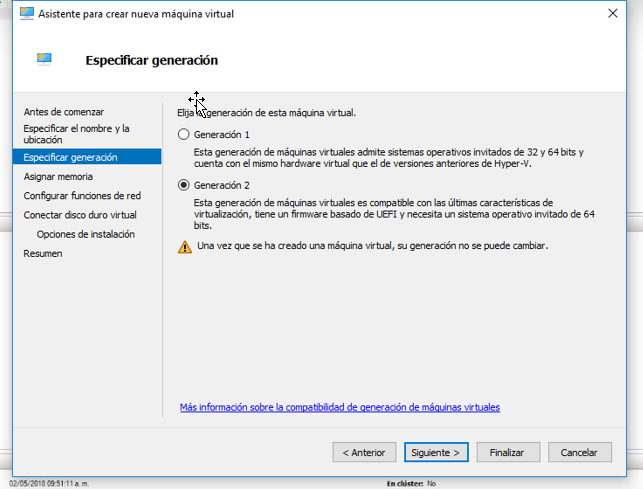
\includegraphics[width=12cm]{./Imagenes/8} 
\end{center}



\begin{itemize}
- Asignamos un total de 4096 MB de memoria RAM\\
\end{itemize}

\begin{center}
	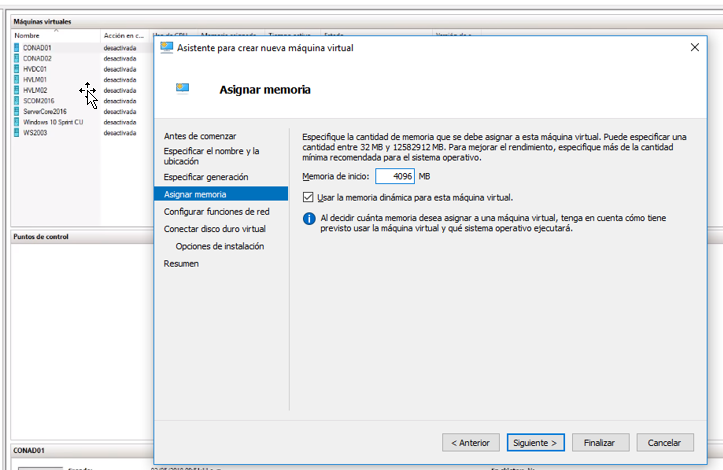
\includegraphics[width=12cm]{./Imagenes/9} 
\end{center}


\begin{itemize}
- En esta parte asignamos la red que hemos creado anteriormente, que en esta ocasión esta con el nombre de 'rednueva'\\
\end{itemize}

\begin{center}
	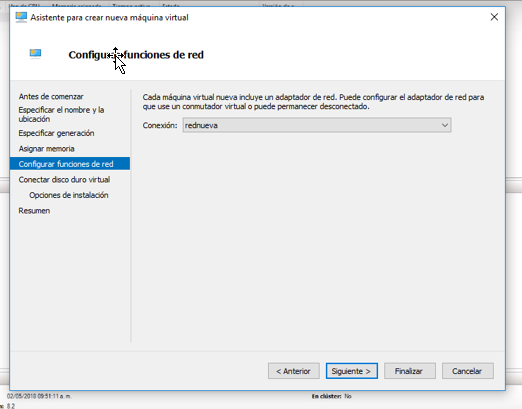
\includegraphics[width=12cm]{./Imagenes/10} 
\end{center}

\begin{itemize}
- En esta ventana escogemos la opción de 'Crear un disco duro virtual', en ubicación elegimos la carpeta donde querer guardar, damos click en siguiente.\\
\end{itemize}

\begin{center}
	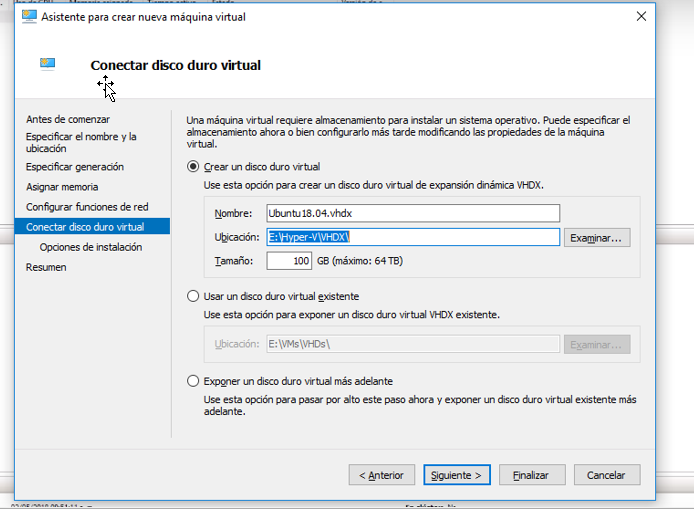
\includegraphics[width=12cm]{./Imagenes/11} 
\end{center}


\begin{itemize}
- En opciones de instalación seleccionamos la imagen .iso de Ubuntu\\
\end{itemize}

\begin{center}
	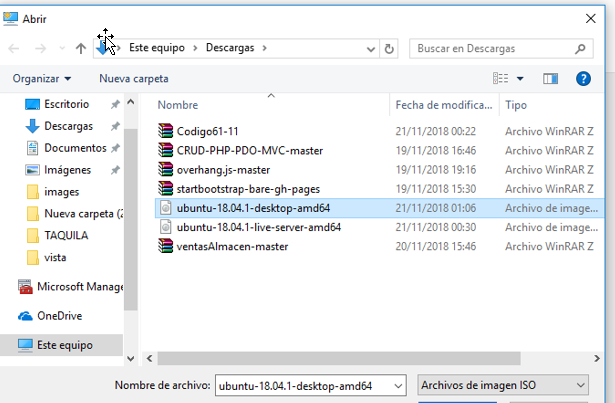
\includegraphics[width=12cm]{./Imagenes/12} 
\end{center}


\begin{itemize}
- Finalizamos la instalación de la maquina virtual\\
\end{itemize}

\begin{center}
	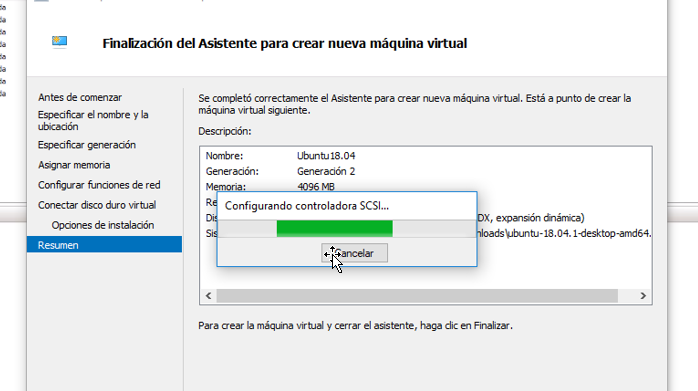
\includegraphics[width=12cm]{./Imagenes/13} 
	
\end{center}


\begin{itemize}
- Antes de iniciar la maquina virtual, vamos a la opcion de configuracion para desabilitar la siguiente opcion\\
\end{itemize}

\begin{center}
	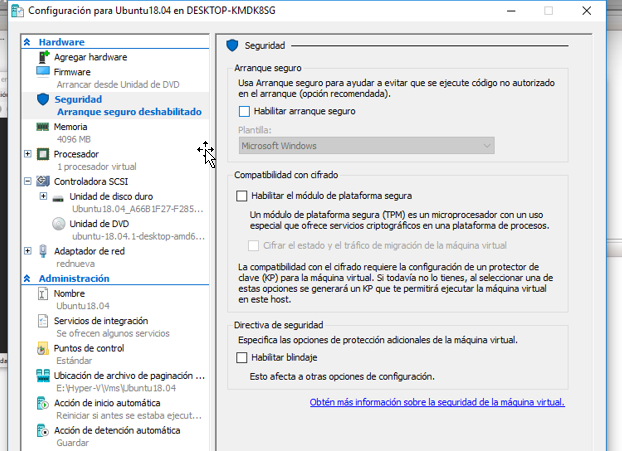
\includegraphics[width=12cm]{./Imagenes/14} 
\end{center}





\begin{itemize}
- Iniciamos la maquina virtual para poder terminar de instalar el sistema operativo Ubuntu, elegimos 'Install Ubuntu'\\
\end{itemize}

\begin{center}
	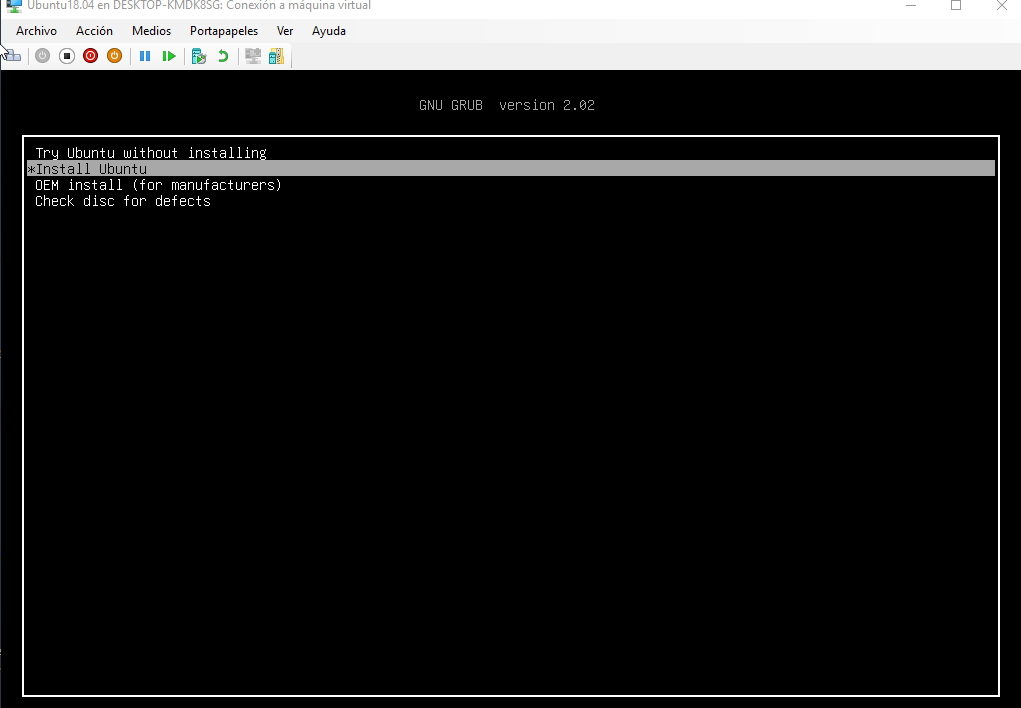
\includegraphics[width=12cm]{./Imagenes/15} 
\end{center}




\begin{itemize}
- Elegimos el idioma, damos continue\\
\end{itemize}

\begin{center}
	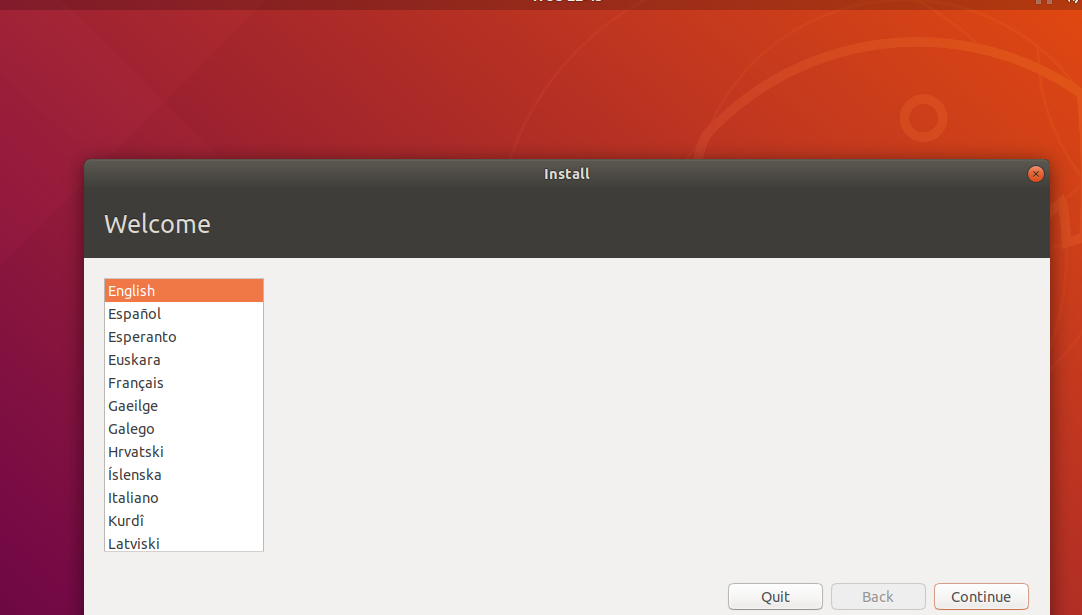
\includegraphics[width=12cm]{./Imagenes/16} 
\end{center}

\begin{itemize}
- Elegimos el idioma del teclado, damos click en continuar\\
\end{itemize}

\begin{center}
	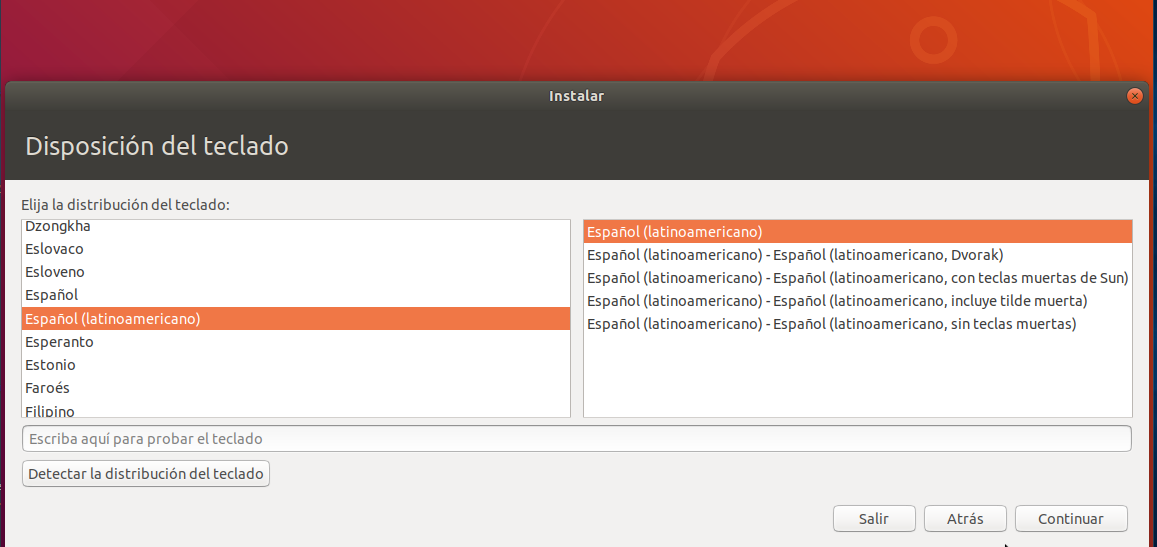
\includegraphics[width=12cm]{./Imagenes/17} 
\end{center}


\begin{itemize}
- En esta parte elegimos 'instalacion normal', damos click en continuar\\
\end{itemize}

\begin{center}
	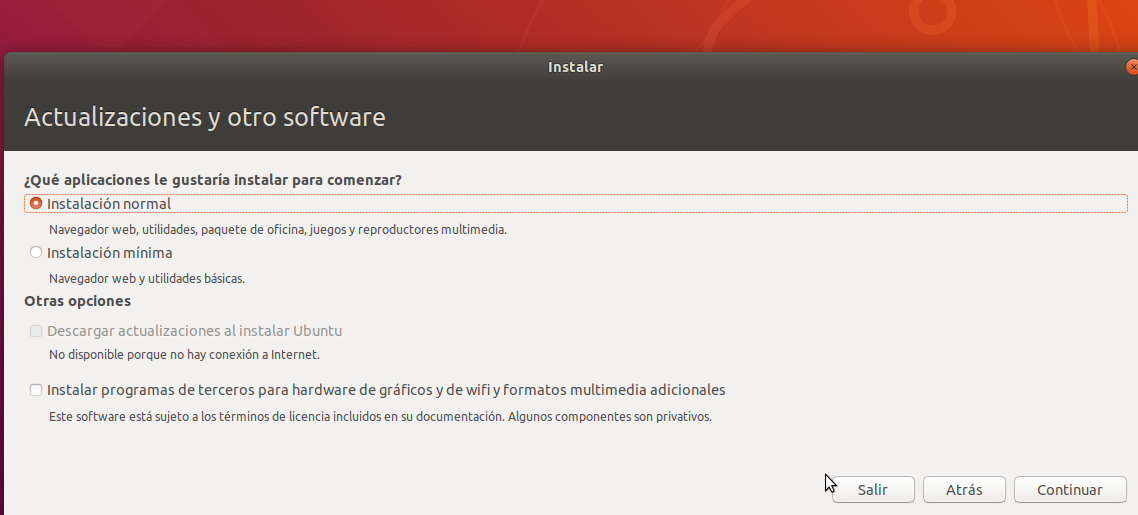
\includegraphics[width=12cm]{./Imagenes/18} 
\end{center}



\begin{itemize}
- Elegimos 'Borrar disco e instalar Ubuntu', y por ultimo damos click en instalar ahora\\
\end{itemize}

\begin{center}
	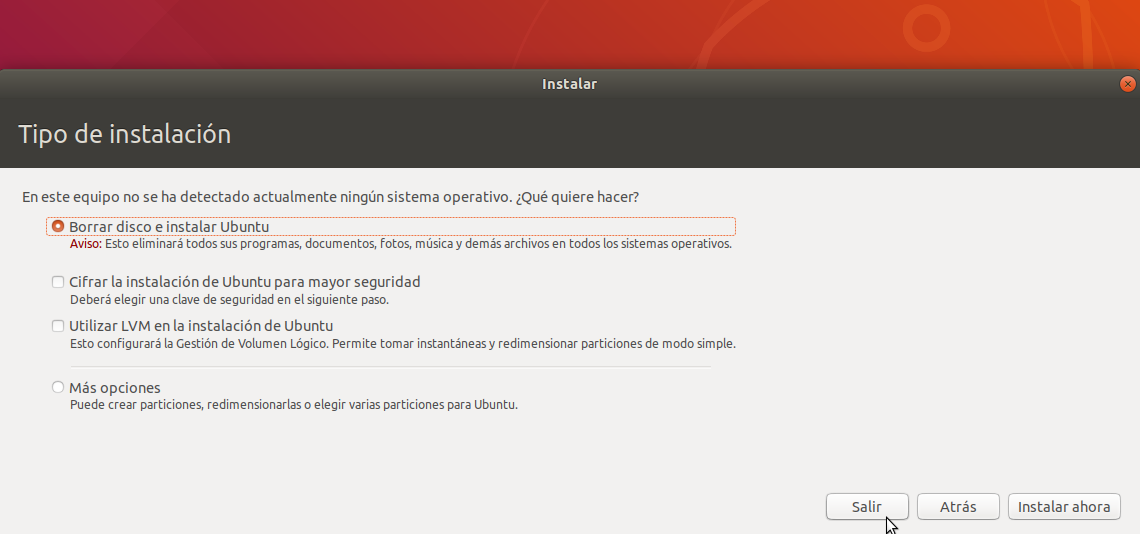
\includegraphics[width=12cm]{./Imagenes/19} 
\end{center}


\begin{itemize}
- Seleccionamos nuestra zona horaria, click en continuar\\
\end{itemize}

\begin{center}
	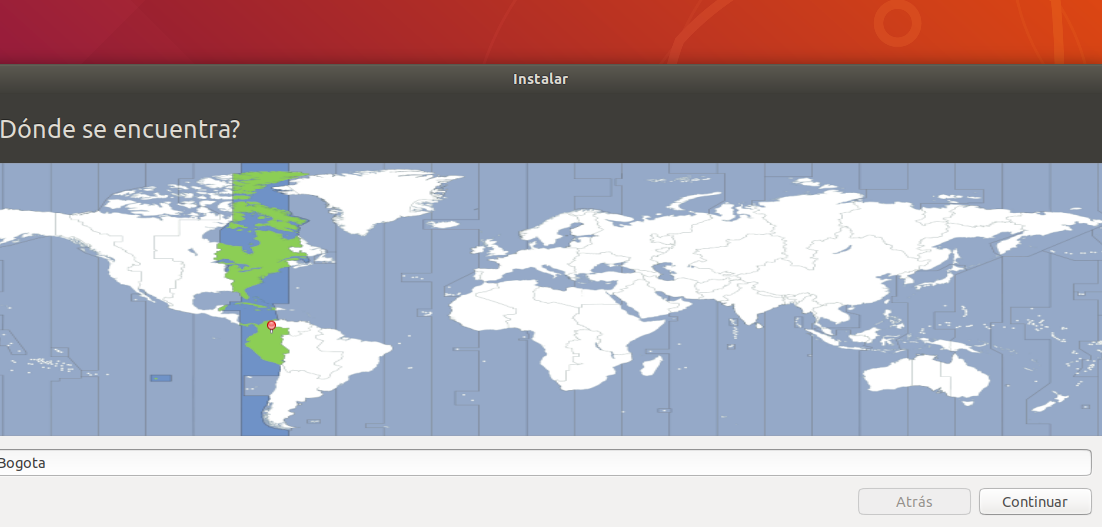
\includegraphics[width=12cm]{./Imagenes/20} 
\end{center}



\begin{itemize}
- Ponemos los datos necesarios que nos piden y esperamos q termine la instalacion\\
\end{itemize}

\begin{center}
	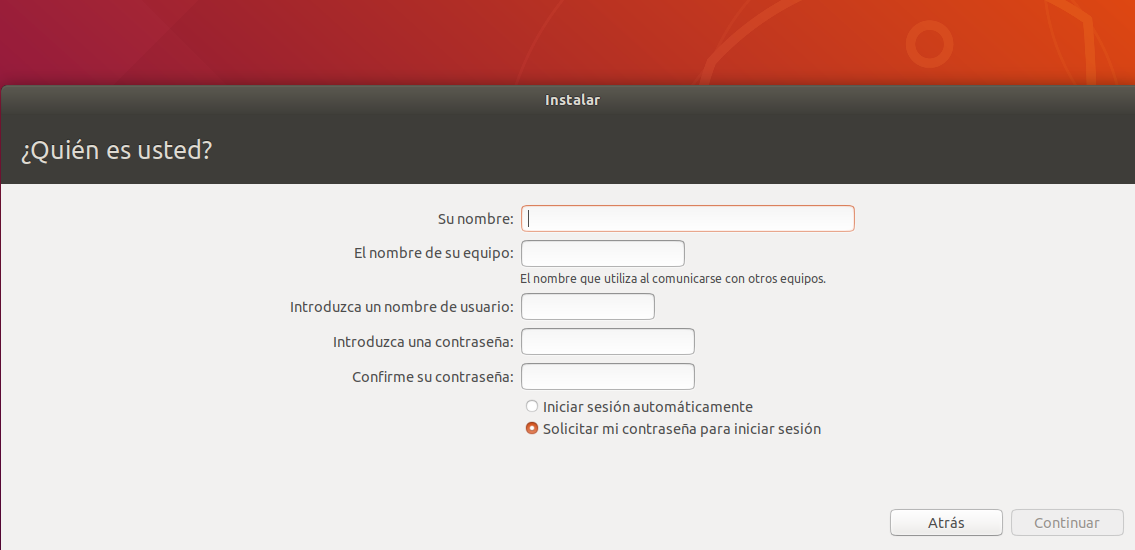
\includegraphics[width=12cm]{./Imagenes/21} 
\end{center}

\begin{itemize}
\subsection{Instalación de Oracle Database Server}\\
- En el sistema Operativo que hemos virtualizamos que en este caso es Ubuntu Linux, iniciamos sesion con el respectivo login y contraseña.
\end{itemize}

\begin{center}
	
\includegraphics[width=10cm]{./Imagenes/22} 
\end{center}


\begin{itemize}
- Verificamos que tengamos todo los software necesarios para la instalacion de database oracle\\
\end{itemize}

\begin{center}
	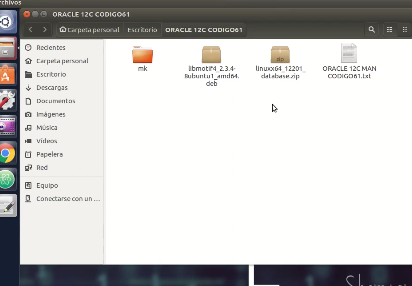
\includegraphics[width=12cm]{./Imagenes/23} 
\end{center}



\begin{itemize}
- En el terminal iniciamos como super usuario para no tener problemas luego descomprimimos el oracle en la carpeta que deseamos de la siguiente manera\\
\end{itemize}

\begin{center}
	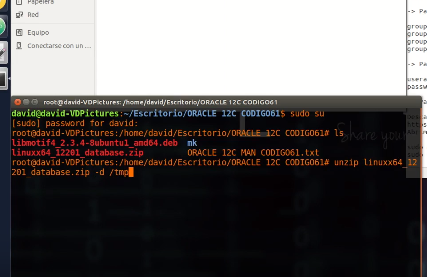
\includegraphics[width=12cm]{./Imagenes/24} 
\end{center}


\begin{itemize}
- En el terminal ponemos el siguiente codigo para crear usuarios\\
\end{itemize}

\begin{center}
	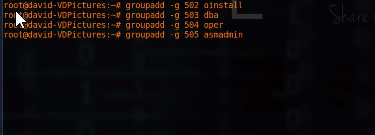
\includegraphics[width=12cm]{./Imagenes/25} 
\end{center}



\begin{itemize}
- Para poder crear usuario para el oracle ponemos que siguiente codigo en el terminal y ponemos la contraseña que deseamos\\
\end{itemize}

\begin{center}
	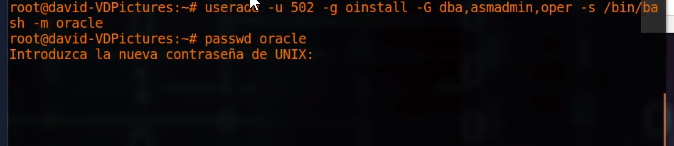
\includegraphics[width=12cm]{./Imagenes/26} 
\end{center}

\begin{itemize}
- Abrimos otro terminal y ponemos el siguiente codigo\\
\end{itemize}

\begin{center}
	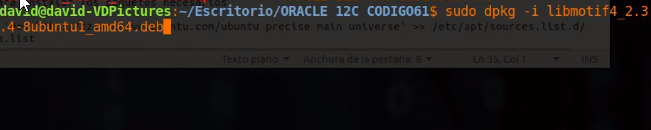
\includegraphics[width=12cm]{./Imagenes/27} 
\end{center}


\begin{itemize}
- Para poder corregir el error ponemos lo siguiente\\
\end{itemize}

\begin{center}
	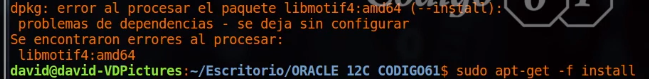
\includegraphics[width=12cm]{./Imagenes/28} 
\end{center}


\begin{itemize}
- Para instalar los paquetes necesarios usamos el siguiente comando\\
\end{itemize}

\begin{center}
	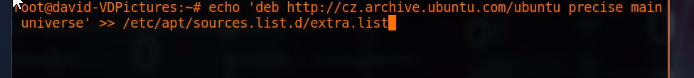
\includegraphics[width=12cm]{./Imagenes/29} 
\end{center}


\begin{itemize}
- Luego el siguiente comando\\
\end{itemize}

\begin{center}
	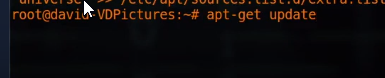
\includegraphics[width=12cm]{./Imagenes/30} 
\end{center}


\begin{itemize}
- Despues ponemos la siguiente linea de codigo y damos en la opcion si\\
\end{itemize}

\begin{center}
	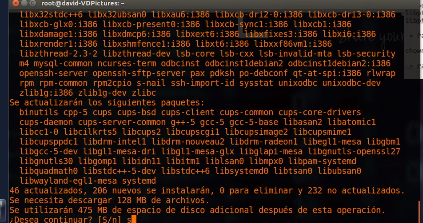
\includegraphics[width=12cm]{./Imagenes/31} 
\end{center}


\begin{itemize}
- Para dar permisos a oinstall para acceder a la instalacion de oracle ponemos el siguiente comando\\
\end{itemize}

\begin{center}
	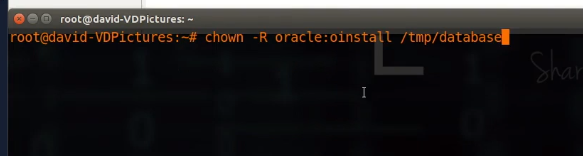
\includegraphics[width=12cm]{./Imagenes/32} 
\end{center}




\begin{itemize}
- Para dar acceso a xhost\\
\end{itemize}

\begin{center}
	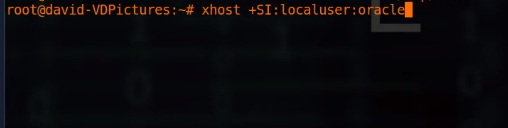
\includegraphics[width=12cm]{./Imagenes/33} 
\end{center}


\begin{itemize}
- Para linkear a binarios y librerias\\
\end{itemize}

\begin{center}
	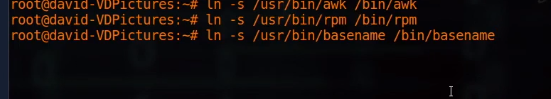
\includegraphics[width=12cm]{./Imagenes/34} 
\end{center}


\begin{itemize}
- luego el siguiente comando\\
\end{itemize}

\begin{center}
	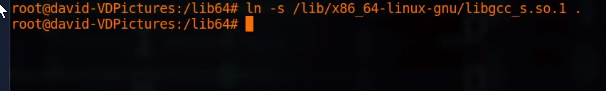
\includegraphics[width=12cm]{./Imagenes/35} 
\end{center}


\begin{itemize}
- Para crear el directorio que contradrá oracle\\
\end{itemize}

\begin{center}
	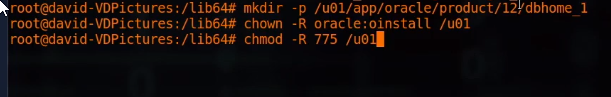
\includegraphics[width=12cm]{./Imagenes/36} 
\end{center}



\begin{itemize}
- Para agregar los parametros del kernel entramos al siguiente archivo nano/etc/sysctl.conf, debe quedar de la siguiente manera\\
\end{itemize}

\begin{center}
	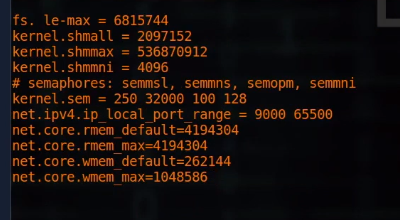
\includegraphics[width=12cm]{./Imagenes/37} 
\end{center}


\begin{itemize}
- Para configurar los parametros del usuario de oracle nos dirigimos a /etc/security/limits.conf, debe quedar de la siguiente manera\\
\end{itemize}

\begin{center}
	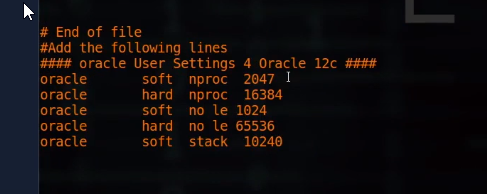
\includegraphics[width=12cm]{./Imagenes/38} 
\end{center}


\begin{itemize}
- Para agregar las rutas de oracle (iniciamos como usuario oracle), nos dirigimos al siguiente archivo, debe quedar de la siguiente manera\\
\end{itemize}

\begin{center}
	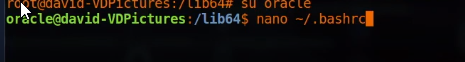
\includegraphics[width=12cm]{./Imagenes/39} 
\end{center}



\begin{itemize}
- Cargamos los nuevos parametros del kernel\\
\end{itemize}

\begin{center}
	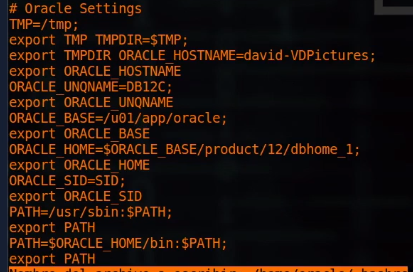
\includegraphics[width=12cm]{./Imagenes/40} 
\end{center}



\begin{itemize}
- Para cargar la nueva configuracion de .bashrc\\
\end{itemize}

\begin{center}
	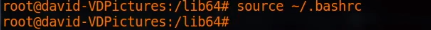
\includegraphics[width=12cm]{./Imagenes/42} 
\end{center}


\begin{itemize}
- Para empezar la instalacion ejecutamos el siguiente comando\\
\end{itemize}

\begin{center}
	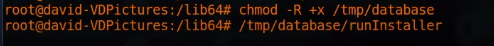
\includegraphics[width=12cm]{./Imagenes/43} 
\end{center}


\begin{itemize}
- Se abrirá el menú de instalación, escribiremos un correo y desmarcaremos el check, presionamos siguiente \\
\end{itemize}

\begin{center}
	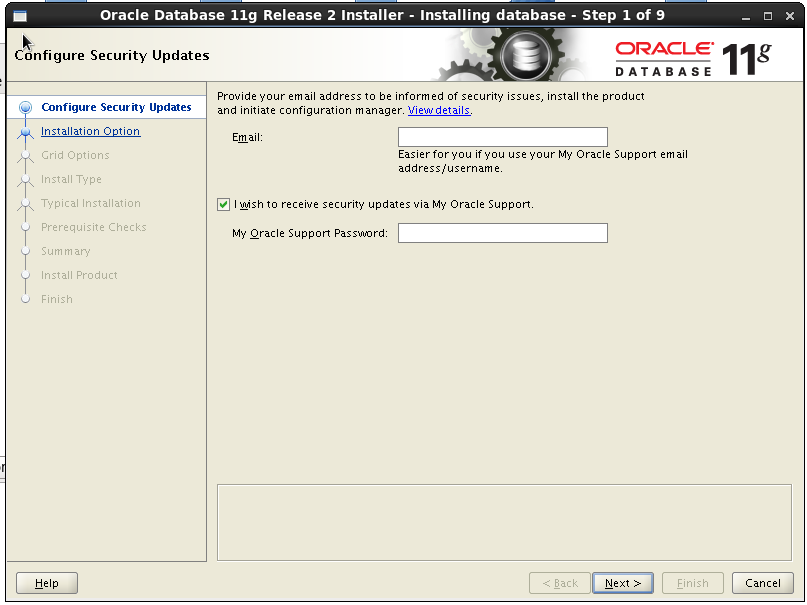
\includegraphics[width=12cm]{./Imagenes/44} 
\end{center}


\begin{itemize}
- Luego nos mostrará la siguiente imagen y selecciamos la primera opción  \\
\end{itemize}

\begin{center}
	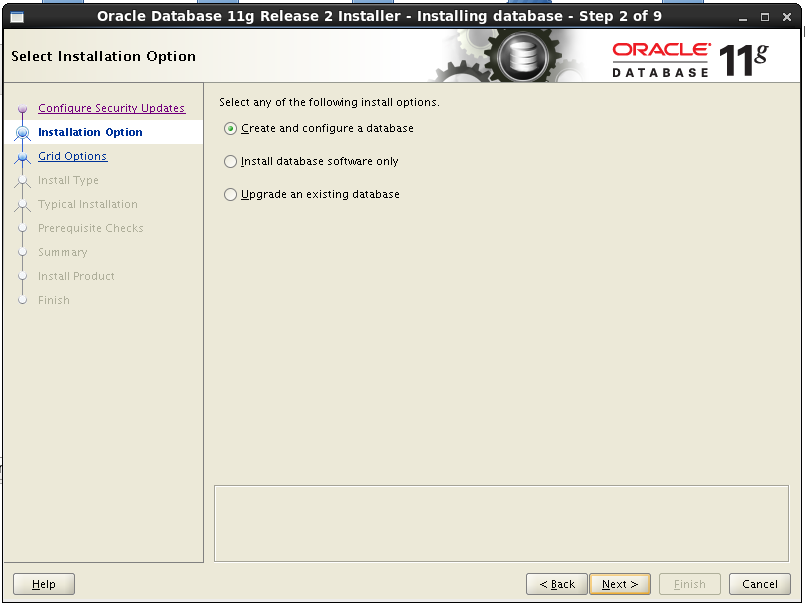
\includegraphics[width=12cm]{./Imagenes/45} 
\end{center}

\begin{itemize}
- Dejamos la opción marcado por defecto \\
\end{itemize}

\begin{center}
	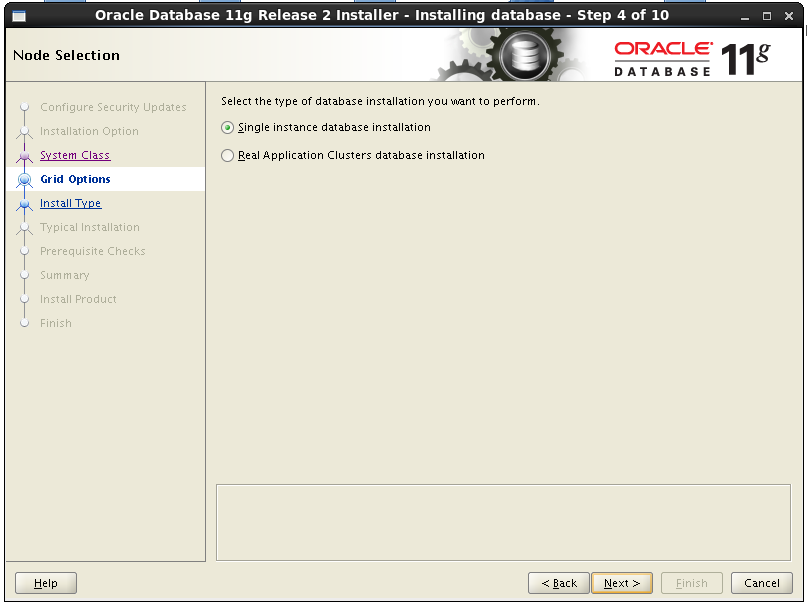
\includegraphics[width=12cm]{./Imagenes/46} 
\end{center}

\begin{itemize}
- En este paso dejamos marcado la opción por defecto, presionamos continuar \\
\end{itemize}

\begin{center}
	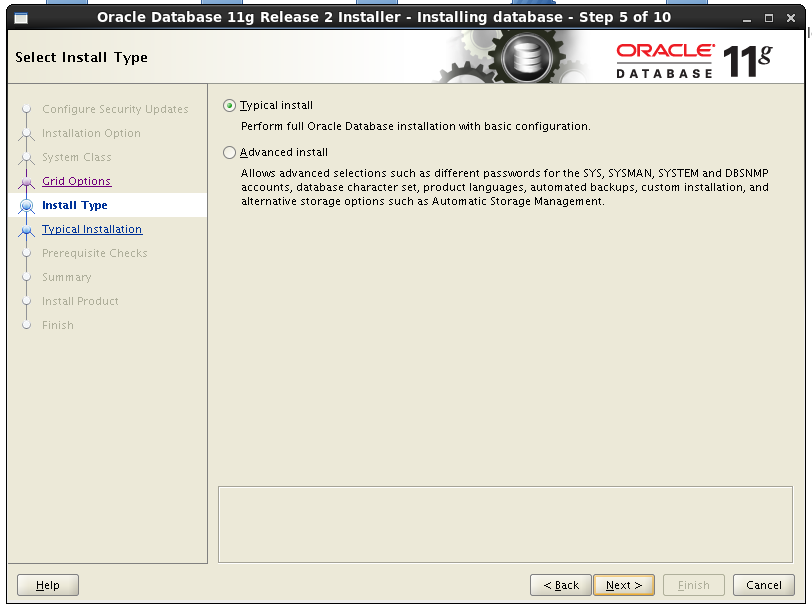
\includegraphics[width=12cm]{./Imagenes/47} 
\end{center}


\begin{itemize}
- Una vez llegado a este paso, tendremos que llenar datos necesarios para continuar \\
\end{itemize}

\begin{center}
	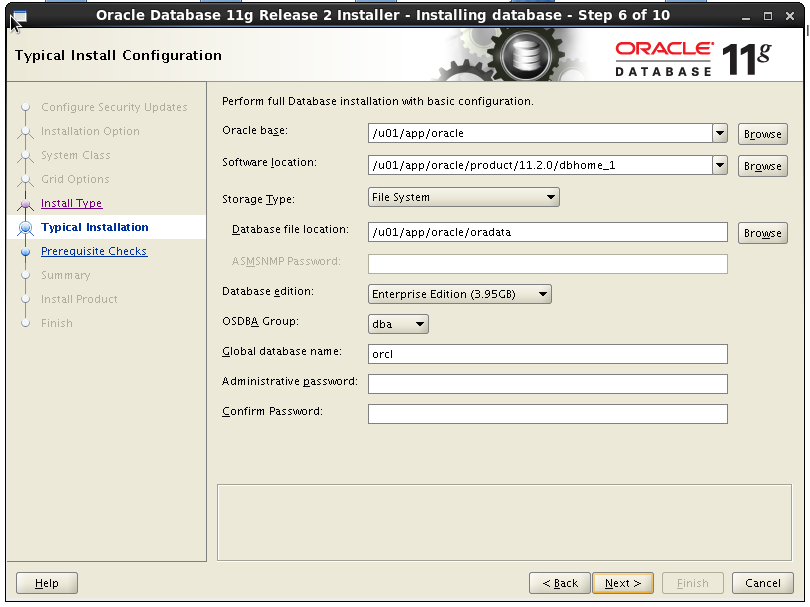
\includegraphics[width=12cm]{./Imagenes/48} 
\end{center}

\begin{itemize}
- Marcamos la casilla que esta en la esquina superior derecha, hacemos click en continuar \\
\end{itemize}

\begin{center}
	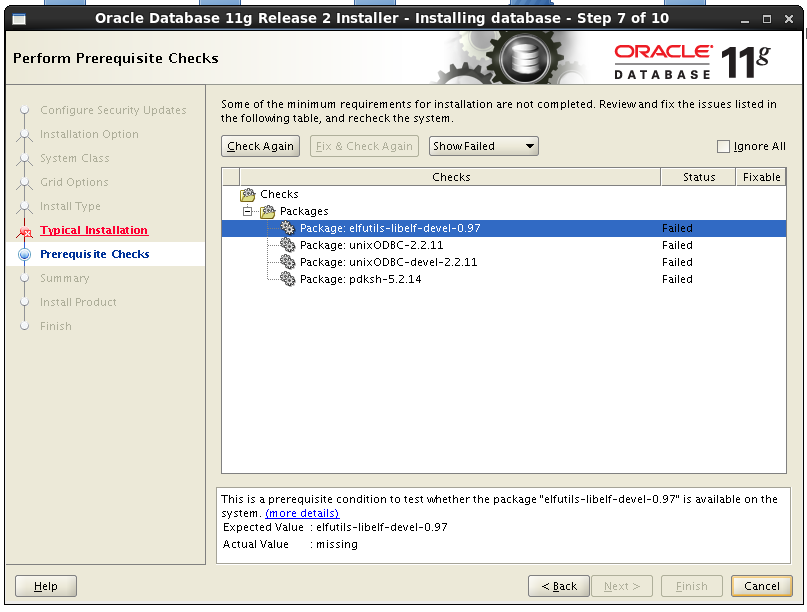
\includegraphics[width=12cm]{./Imagenes/49} 
\end{center}

\begin{itemize}
- Al terminar la instalación nos mostrará esta imagen \\
\end{itemize}

\begin{center}
	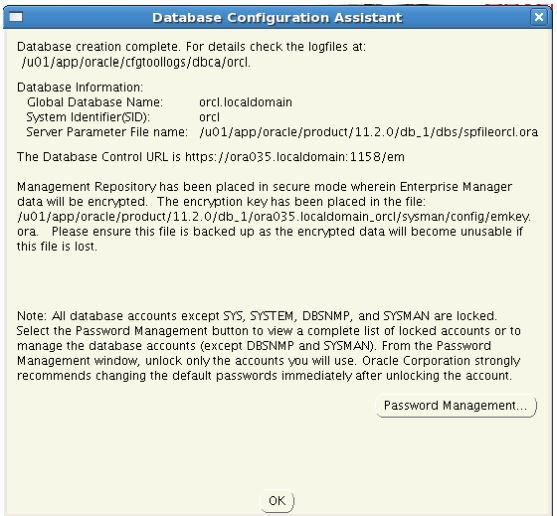
\includegraphics[width=12cm]{./Imagenes/50} 
\end{center}


\begin{itemize}
- Luego nos mostrará una ventan, cambiamos de usuario a root y copiamos las dos rutas en una terminal \\
\end{itemize}

\begin{center}
	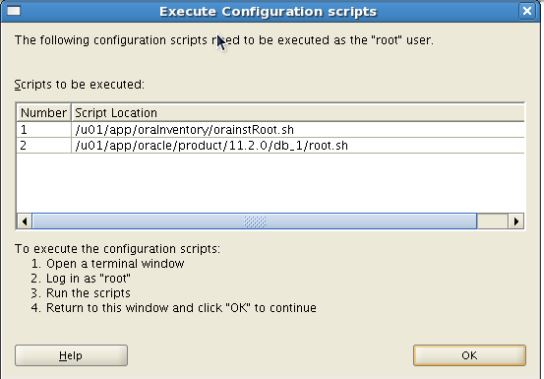
\includegraphics[width=12cm]{./Imagenes/51} 
\end{center}


\begin{itemize}
- Por ultimo abrimos un navegador, ponemos la siguiente dirección para poder ingresar al gestor de base de datos oracle \\
\end{itemize}

\begin{center}
	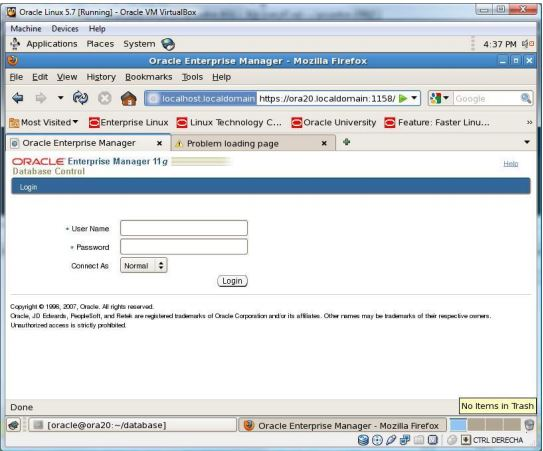
\includegraphics[width=12cm]{./Imagenes/52} 
\end{center}

\end{document}